\documentclass{VUMIFPSkursinis}
\usepackage{algorithmicx}
\usepackage{algorithm}
\usepackage{algpseudocode}
\usepackage{amsfonts}
\usepackage{amsmath}
\usepackage{bm}
\usepackage{caption}
\usepackage{color}
\usepackage{float}
\usepackage{graphicx}
\usepackage{listings}
\usepackage{subfig}
\usepackage{wrapfig}

\usepackage{enumitem}
%PAKEISTA, tarpai tarp sąrašo elementų
\setitemize{noitemsep,topsep=0pt,parsep=0pt,partopsep=0pt}
\setenumerate{noitemsep,topsep=0pt,parsep=0pt,partopsep=0pt}

% Titulinio aprašas
\university{Vilniaus universitetas}
\faculty{Matematikos ir informatikos fakultetas}
\department{Programų sistemų katedra}
\papertype{Programų sistemų inžinerijos I laboratorinis darbas Nr. 1}
\title{Kavinės staliuko rezervavimo aplikacija}
\titleineng{Cafe table rezervation app}
\status{2 kurso 5 grupės studentai}
\author{Paulius Grigaliūnas}
\secondauthor{Karolis Staskevičius}
\thirdauthor{Modestas Dulevičius}
\fourthauthor{Albert Jurkoit}
\fifthauthor{Šarūnas Kazimieras Buteikis}
     

% \secondauthor{Vardonis Pavardonis}   % Pridėti antrą autorių
\supervisor{dr. Vytautas Valaitis}
\date{Vilnius – \the\year}

% Nustatymai
% \setmainfont{Palemonas}   % Pakeisti teksto šriftą į Palemonas (turi būti įdiegtas sistemoje)
\bibliography{bibliografija}

\begin{document}
	
% PAKEISTA	
\maketitle
\cleardoublepage\pagenumbering{arabic}
\setcounter{page}{2}


%ANOTACIJA

\sectionnonum{ANOTACIJA}
{\bfseries Darbo tikslas:} sukurti išmanų, patogų kavinių staliukų rezervavimo programėlės modelį, kuris funkcionuotų Windows ir Android sistemose. Taip pat siekiama, kad galutinė programėlė užtikritnų sklandų, spartų komunikabilumą tarp klientų ir kavinės darbuotojų, suteikiant galimybę kavinių savininkams pateikti išsamų kavinės planą, o klientams išsirinkti norimą staliuką kavinėje patiems. 
\newline
\newline
\newline

%DARBO ATLIKO

{\bfseries Darbą atliko:}
\newline
\newline
\newline
Paulius Grigaliūnas
\newline
paulius.grigaliunas.pg@gmail.com
\newline
\newline
\newline
Karolis Staskevičius
\newline
karolio paštas
\newline
\newline
\newline
Modestas Dulevičius
\newline
modux9@gmail.com
\newline
\newline
\newline
Albert Jurkoit
\newline
albert.jurkoit@mif.stud.vu.lt
\newline
\newline
\newline
Šarūnas Kazimieras Buteikis
\newline
sarunas.kazimieras.buteikis@gmail.com

%TURINYS

\tableofcontents

%ĮVADAS

\sectionnonum{Įvadas}
\noindent
{\bfseries "Book a Table" kavinės rezervavimo aplikacija}
\newline
\newline
{\bfseries Dalykinė sritis}
\newline
Kavinės ir jų rezervacija
\newline
\newline
{\bfseries Probleminė sritis}
\newline
 Lietuvoje staliuko rezervavimo galimybės yra mažai praplėstos
\newline
\newline
{\bfseries Naudotojai}
\newline
Žmonės, norintys skaniai pavalgyt, bei iš anksto pasirūpint vietą restorane.
\newline
Kavynių savininkai, suteikiantys žmonėms galimybę rezervuoti staliuką jų restorane.
\newline
\newline
{\bfseries Darbo pagrindas}
\newline
Dokumentas parengtas kaip programų sistemų inžinerios dalyko laboratorinis darbas Nr. 1, kuriame pateikiamas suprojektuotos sistemos aprašymas.
\newline
\newline

\section{Programų sistemos architektūra}
%LOGINIS PJUVIS
\subsection{Loginis pjūvis}
%KLASIU DIAGRAMA
\subsubsection{Klasių diagrama}



Žemiau pateiktoje klasių diagromoje (1 pav.) yra išskirtos pagrindinės esybės, kurios yra naudojamos sistemoje. Klases siejantys ryšiai pasižymi kardinalumu, t.y. nustatytas konkretus ryšių skaičius, kuriuos turės klasės egzempliorius su kitomis klasės egzemplioriais.
\newline
\newline

\begin{figure}[H]
    \centering
    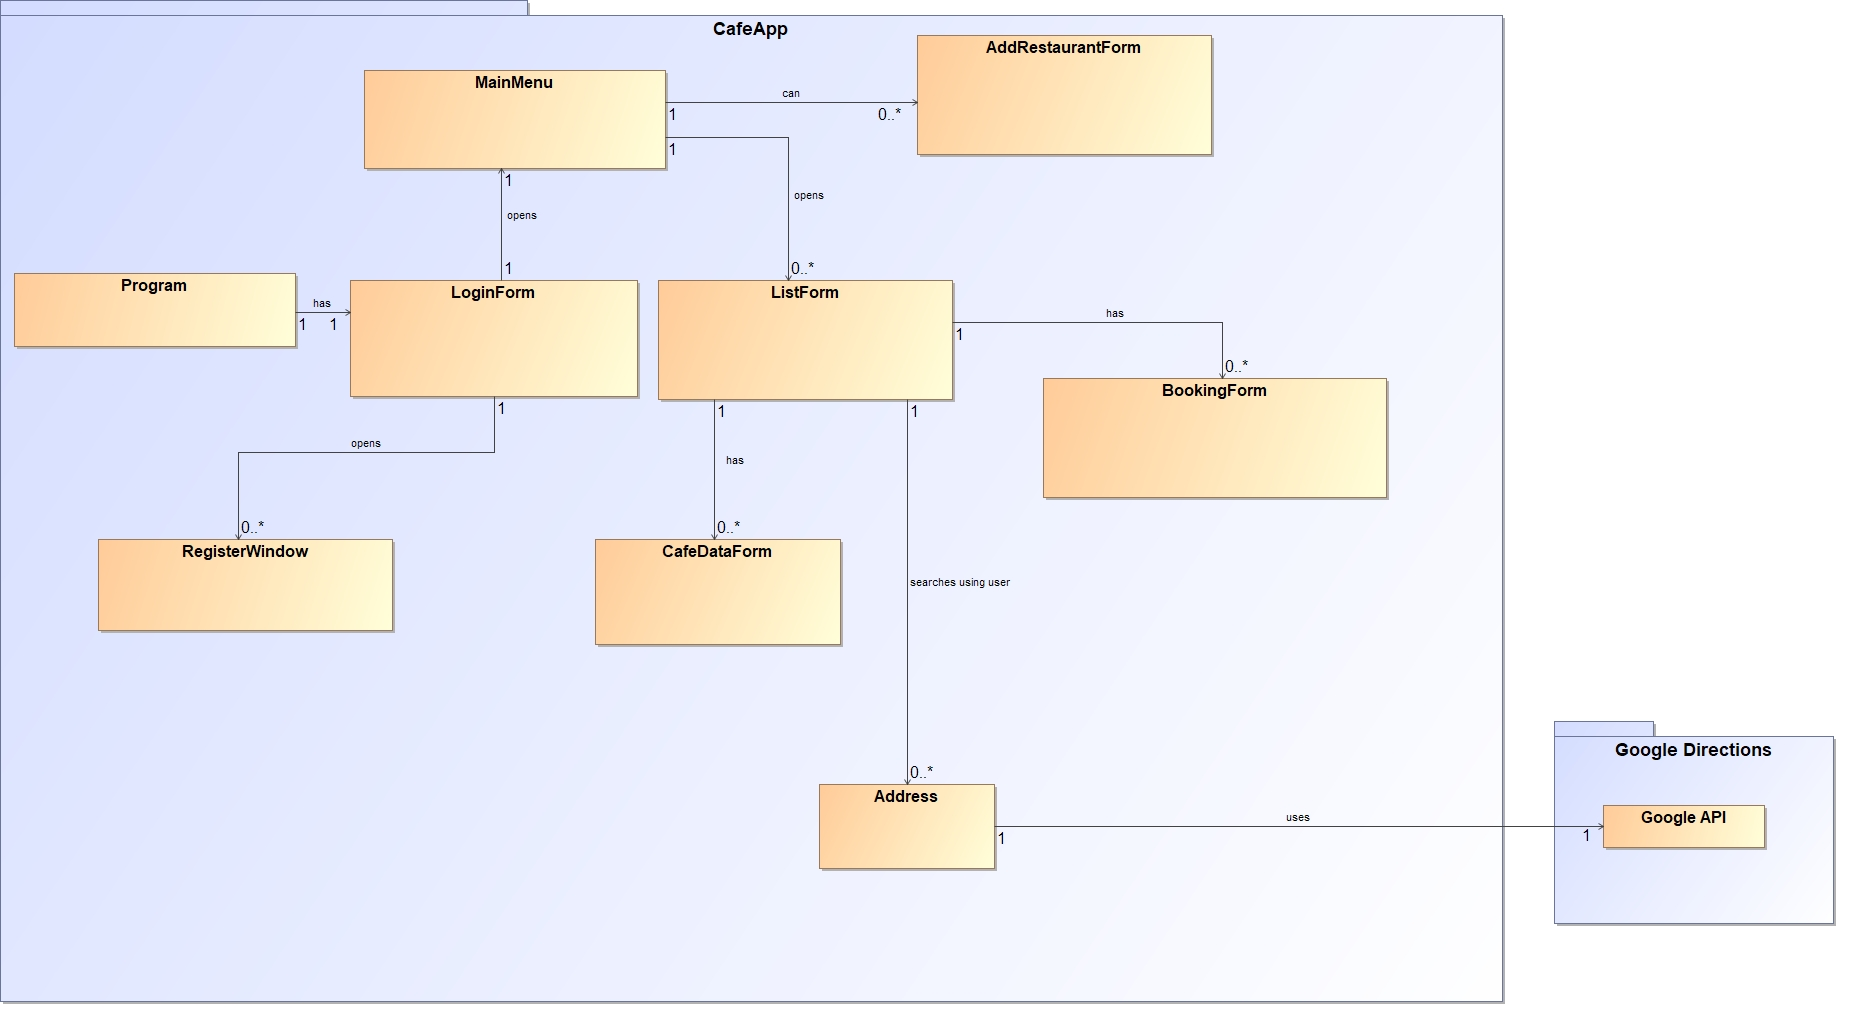
\includegraphics[width=\textwidth,height=\textheight,keepaspectratio]{img/Model} 
    \caption{Klasių diagrama}
    \label{img:Model}
\end{figure}
%1 PAV APRAŠYMAS
Pateiktoje diagramoje yra visos programos sistemos modelis. Programa galima suskirstyti į 3 dalis: vartotojo prisijungimas/registracija prie aplikacijos, kavinių registravimas bei registruotų kavinių sąrašas ir kavinių paieška, rezervavimas ir kavinės informacijos modifikavimas. Apie jas bus plačiau aprašome kitose klasių diagramose.
\pagebreak
%2 PAV APRAŠYMAS

Paleidus programą (2 pav.) vartotojas gali prisijungti arba sukurti naują paskyrą. Mes nusprendemė, kad vartotojui, nuėjus į naujos paskyros langelį nedingtų pradinis langelis. Tokiu būdu vartotojui užsiregistravus bus galima iš karto prisijungti ir atsidurti mūsų programos pagrindiniame langelyje arba sukurti naują paskyrą, jeigu jis būtų nepatenkintas esama paskyra. 
\newline
\newline
\newline
\newline
\newline
\newline
\begin{figure}[H]
    \centering
    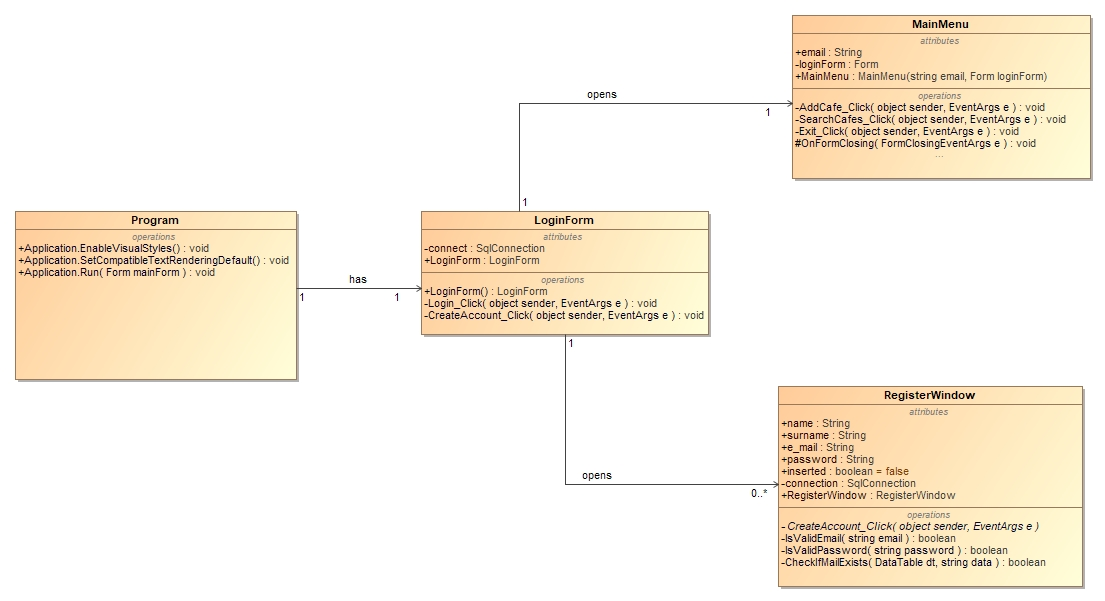
\includegraphics[width=\textwidth,height=\textheight,keepaspectratio]{img/Program_LoginForm_Register_MainMenu} 
    \caption{Programos paleidimo ir vartotojo prisijungimo ir registracijos  klasių diagrama}
    \label{img:Program_LoginForm_Register_MainMenu}
\end{figure}

Kuriant naują paskyrą, privaloma įvesti paštą ir slaptažodį. Bus patikrinama ar įvesti duomenys yra korektiški, taip pat bus patikrinama ar jau nėra tokios sukurtos paskyros su įvestais duomenimis. Prisijungimo metu tikrinama ar yra tokia sukurta paskyra.

\pagebreak
%3 PAV APRAŠMAS
Žemiau pateiktoje klasių diagramoje (3 pav.) pavaizduotos klasės, susijusios su pagrindiniu programos langeliu. Šiame langelyje galima pridėti kavinę į kavinių sąrašą arba atsiverti kavinių sąrašą. Norint pridėti kavinę privaloma nurodyti kavinės pavadinimą, adresą, tvarkaraštį (nuo kada iki kada dirba darbo dienomis, savaitgaliais) ir vartotojo telefono numerį.
\newline
\newline
\newline
\newline
\newline
\newline
\begin{figure}[H]
    \centering
    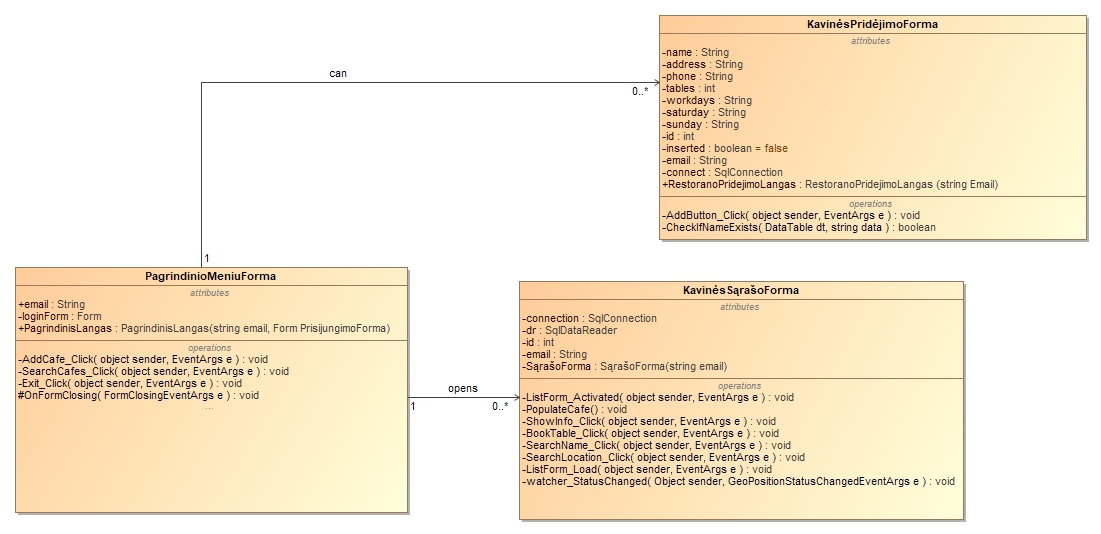
\includegraphics[width=\textwidth,height=\textheight,keepaspectratio]{img/MainMenu_AddRestaurant_ListForm} 
    \caption{kavinių registravimo ir registruotų kavinių sąrašo klasių diagrama}
    \label{img:MainMenu_AddRestaurant_ListForm}
\end{figure}

Kavinės registravimo metu yra patikrinama ar yra kavinė su tokia pačia informacija, kad būtų išvengta dubliavimo.

\pagebreak
%4 PAV APRAŠYMAS
4 pav. klasių diagramoje parodomas kavinių paieška ir kavinės rezervavimas. Mes nusprendėme leisti vartotojui ieškoti norimos kavinės pagal kavinės vardą arba pagal vartotojo esamą vietovę. Taip palengvinama kavinės paieška, jeigu vartotojas žino, jog yra šalia kavinės, bet nežino jos pavadinimo, arba žino kavinės pavadinimą, bet nežino kur ji randasi. Jeigu vartotojas yra ir registruotos kavinės savininkas, jis  gali pakeisti jos vardą, adresą, staliukų skaičių, telefono numerį. Tokiu būdu pataisoma klaidinga registruotos kavinės informacija.
\newline
\newline
\newline
\newline
\newline
\newline
\newline
\newline

\begin{figure}[H]
    \centering
    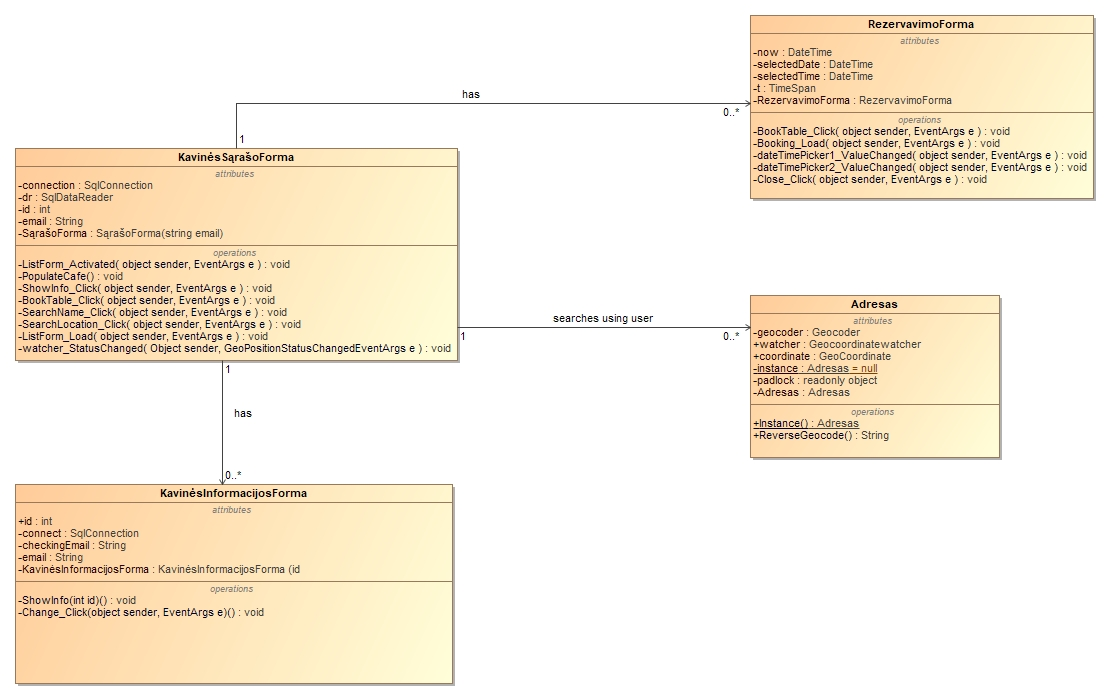
\includegraphics[width=\textwidth,height=\textheight,keepaspectratio]{img/LoginForm_Address_Booking} 
    \caption{kavinių paieškos ir kavininės rezervavimo klasių diagrama}
    \label{img:LoginForm_Address_Booking}
\end{figure}

%Modes use-cases
\subsection{Užduotys ir jų vykdymo scenarijai (angl. Use-cases)}
\subsubsection{Sistemos vykdomos užduotys}

%first figure text
Sistema besinaudojantis vartotojas gali atlikti žemiau pateiktas užduotis. Nusprendėme užduotis išskirstyti į „Paprasto vartotojo“ ir „Restorano savininko“, nes šie agentai turi galimybę atlikti skirtingas užduotis. Restorano savininkas taip pat yra paprastas vartotojas, tačiau savininko statusas leidžia jam tvarkyti tik savo pridėtus restoranus (pvz.: pakeisti restorano informaciją). Paprastas vartotojas taip pat gali tapti restorano savininku, jei prideda savo restoraną. Tai atsispindi žemiau pateiktoje sistemos užduočių diagramoje.

%first picture SystemTasks
\begin{figure}[H]
	\centering
	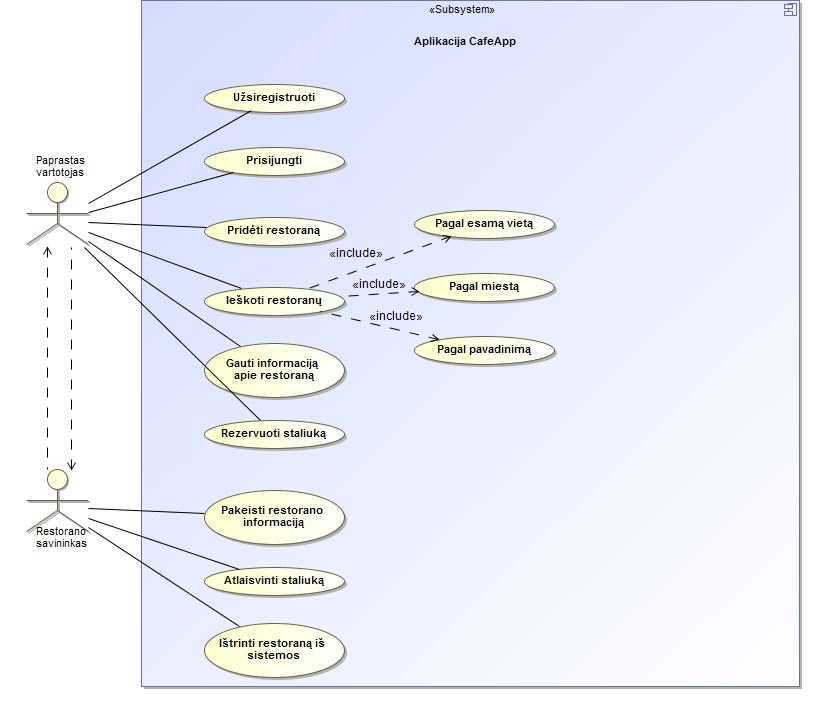
\includegraphics[width=\textwidth,height=\textheight,keepaspectratio]{img/SystemTasks}
	\caption{Sistemos užduočių diagrama}
	\label{img:SystemTasks}
\end{figure}

%second section
\subsubsection{Užduoties „Prisiregistruoti prie sistemos“ vykdymas}
Užduoties „Prisiregistruoti prie sistemos“ sekų diagrama. Vartotojas, naudodamasis GUI, paspaudžia mygtuką „Registruotis“ ir juo iškviečia registracijos formą, kurioje užpildo reikalingus laukus. Duomenys siunčiami kontroleriui, kuris patikrina ar jie tvarkingi (pvz.: ar egzistuoja toks elektroninio pašto adresas), ir iš kontrolerio siunčiama komanda sukurti duomenų bazėje naują įrašą apie vartotoją.

%second figure
\begin{figure}[H]
	\centering
	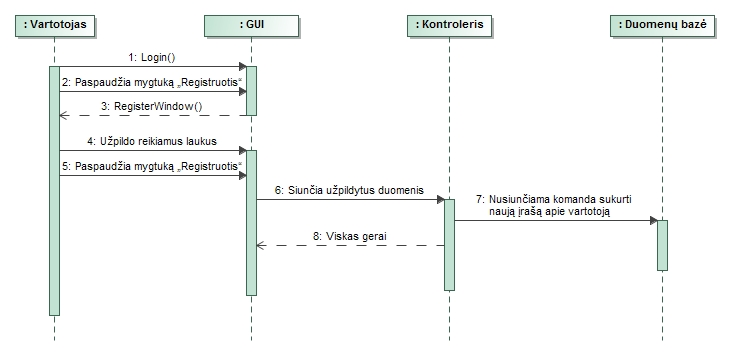
\includegraphics[width=\textwidth,height=\textheight,keepaspectratio]{img/Register}
	\caption{Užduoties „Prisiregistruoti prie sistemos" sekų diagrama}
	\label{img:RegisterTask}
\end{figure}

%third section
\subsubsection{Užduoties „Pridėti naują restoraną“ vykdymas}
Žemiau pateiktoje sekų diagramoje pavaizduotas užduoties „Pridėti naują restoraną“ vykdymas. Vartotojas spaudžia mygtuką „Add a Cafe“ taip iškviesdamas GUI formą, kurią užpildo. Tada paspaudžia mygtuką „Add“ ir duomenys yra validuojami kontroleryje. Jeigu jie neatitinka nustatytų reikalavimų (pvz.: trūksta būtinų užpildyti laukų), vartotojui pranešama ir prašoma pataisyti duomenis. Priešingu atveju, siunčiama užklausa į duomenų bazę, kuri sukuria  naują įrašą, apie pridėtą restoraną, o vartotojas automatiškai tampa restorano savininku.

%third picture
\begin{figure}[H]
	\centering
	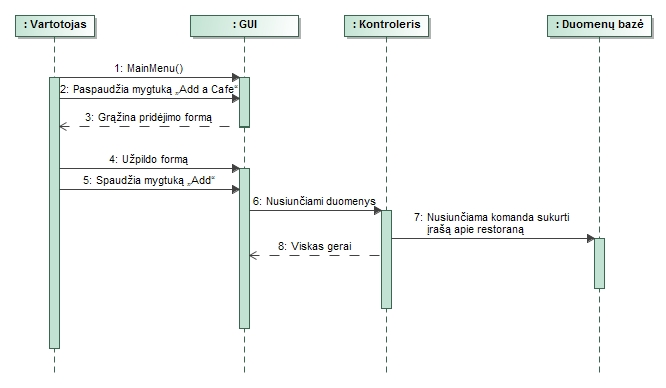
\includegraphics[width=\textwidth,height=\textheight,keepaspectratio]{img/AddRestaurant}
	\caption{Užduoties „Pridėti naują restoraną" sekų diagrama}
	\label{img:AddRestaurant}
\end{figure}

%next section
\subsubsection{Užduoties „Ieškoti restoranų“ vykdymas}
Užduoties „Ieškoti restoranų“ sekų diagrama. Vartotojas paspaudžia mygtuką „Search Cafes“ ir iškviečia naują duomenų formą, kurioje užpildo paieškos kriterijus. Yra numatyti trys kriterijai: pagal esamą vietą, pagal miestą/adresą ir pagal restorano pavadinimą. Duomenys siunčiami kontroleriui, kuris patikrina pateiktus kriterijus, jeigu reikia, nustato esamą vietą, paprašydamas įjungti įrenginio lokaciją. Jeigu viskas yra gerai, siunčiama paieškos užklausa į duomenų bazę ir ji, naudodamasi GUI, pateikia restoranus pagal pasirinktus paieškos laukus. Tai atsispindi žemiau pavaizduotoje sekų diagramoje.

%fourth picture
\begin{figure}[H]
	\centering
	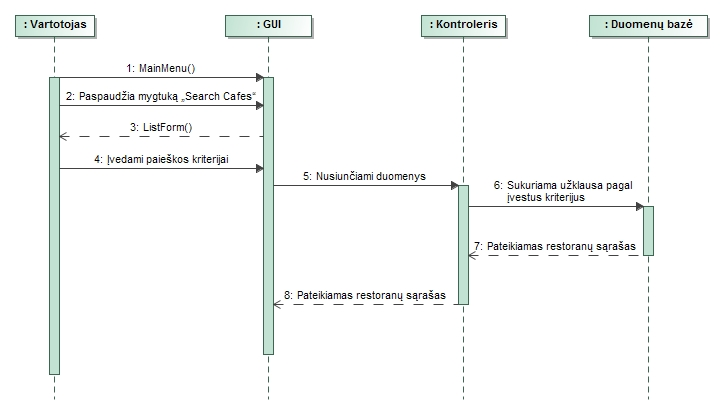
\includegraphics[width=\textwidth,height=\textheight,keepaspectratio]{img/SearchCafes}
	\caption{Užduoties „Ieškoti restoranų" sekų diagrama}
	\label{img:SearchCafes}
\end{figure}

%last section
\subsubsection{Užduoties „Pakeisti restorano informaciją“ vykdymo scenarijus}
Žemiau pavaizduota užduoties „Pakeisti restorano informaciją“ sekų diagrama. Restorano savininkas paspaudžia mygtuką „Search Cafes“ ir juo GUI kreipiasi į duomenų bazę, kuri pateikia visus užregistruotus restoranus. Vykdydamas užduotį „Ieškoti restoranų“ savininkas susiranda savo restoraną, jį pažymėdamas kairiuoju pelės klavišu. Tada paspaudžia mygtuką „Show Info“ ir GUI iškviečia naują formą, kuri kreipiasi į duomenų bazę pagal restorano „ID“ ir parodo informaciją apie restoraną. Joje yra tušti laukai, kuriuos užpildydamas vartotojas gali pakeisti tam tikrą restorano informaciją. Mygtuku „Change“ vartotojas kreipiasi į kontrolerį, kuris siunčia užklausą į duomenų bazę, patikriną, ar būtent šis vartotojas sukūrė įrašą apie restoraną, ir jeigu tai tiesa, vėl kreipiamasi į duomenų bazę - atnaujinti pakeistus duomenis. Jeigu vartotojas neturi teisės keisti informacijai, jam apie tai pranešama.

%last picture
\begin{figure}[H]
	\centering
	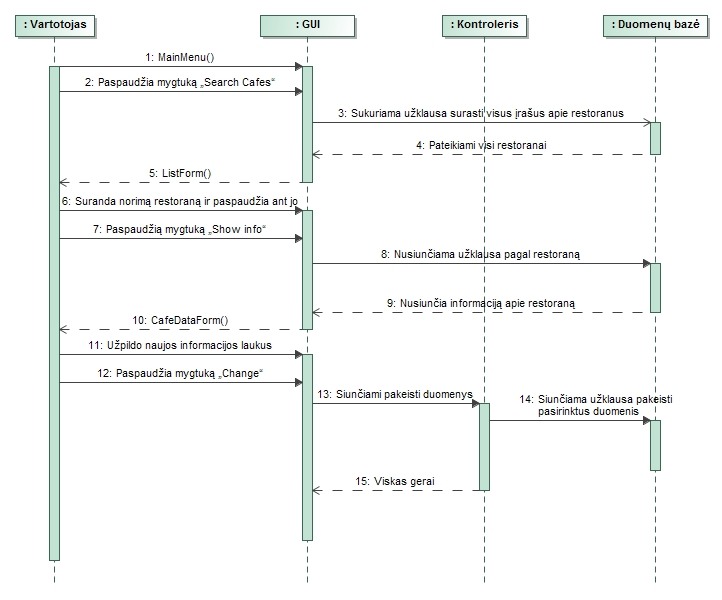
\includegraphics[width=\textwidth,height=\textheight,keepaspectratio]{img/ChangeInfo}
	\caption{Užduoties „Pakeisti restorano informaciją" sekų diagrama}
	\label{img:ChangeInfo}
\end{figure}
%Baigias Modes failai

\subsection{Dinaminis programų sistemos modelis (angl. Process view)}
\subsubsection{Veiklos diagramos}
\begin{figure}[H]
    \centering
    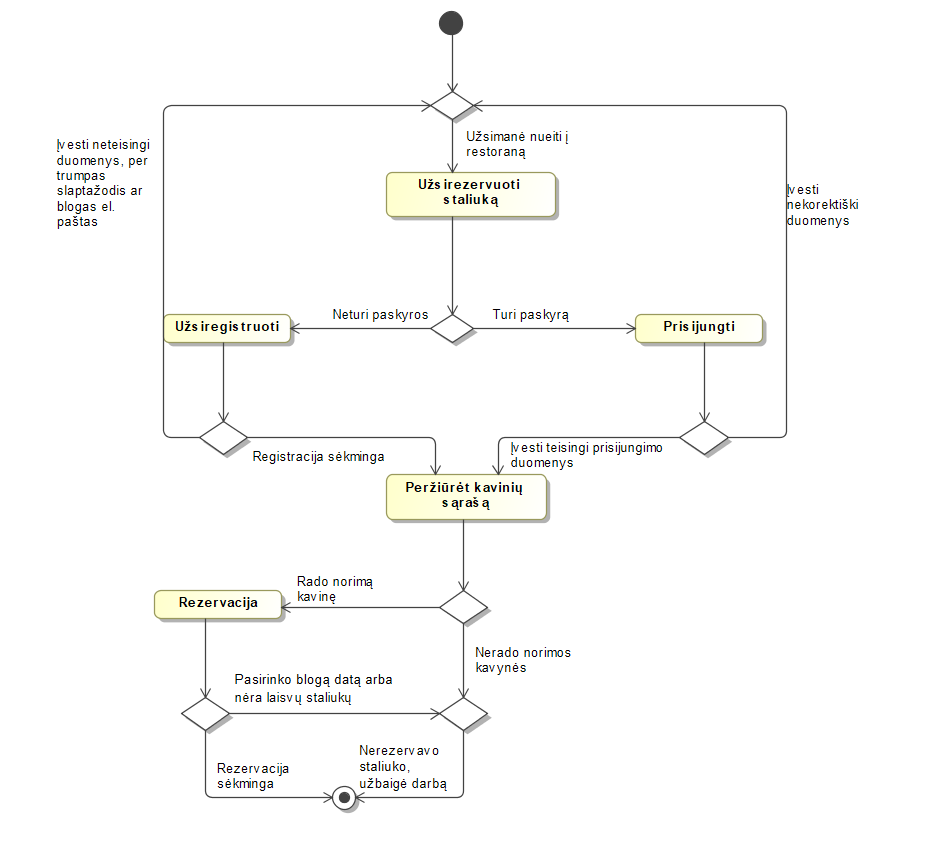
\includegraphics[width=\textwidth,height=\textheight,keepaspectratio]{img/rezerv} 
    \caption{Kavinės rezervacijos veiklos diagrama}
    \label{img:rezerv}
\end{figure}
% Vietoj x įrašyt real sk.
x pav.   diagramoje nagrinėjami procesai, vykstantys tuo metu, kai vartotojas nori rezervuoti staliuką kavinėje. Rezervacija yra pasiekiama tik po prisijungimo arba užsiregistravimo sistemoje. Vartotojas pamato prisijungimo ir registracijos opcijas tik paleidęs aplikaciją. Būsimas sistemos narys privalo užpildyti registracijos formą, parinkti saugų slaptažodį, bei nurodyt egzistuojantį el. paštą. Užpildžius formą neteisingai, reikia pakeisti netinkamus laukus. Sėkmingai prisijungus prie sistemos, vartotojas gali peržiūrėti aplikacijoje užregistruotų kavinių sąrašą. Jeigu vartotojas randa jam patinkančią kavinę, jis užpildo rezervavimo formą. Jeigu formoje visi laukai yra nurodyti teisingai ir restorane yra laisvų staliukų - rezervacija yra sėkminga. Darbas yra baigiamas tuo metu, kai vartotojas sėkmingai užsirezervavo staliuką, arba nusprendė nutraukt rezervaciją.


\begin{figure}[H]
    \centering
    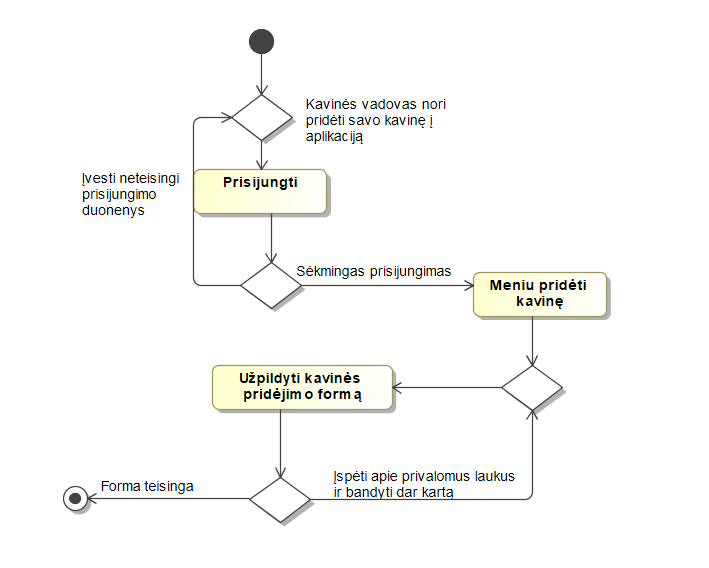
\includegraphics[width=\textwidth,height=\textheight,keepaspectratio]{img/addcafe} 
    \caption{Kavinės pridėjimo prie sistemos veiklos diagrama}
    \label{img:addcafe}
\end{figure}
% Vietoj x įrašyt real sk.
x pav.   diagramoje nagrinėjami procesai, vykstantys vartotojui į sistemą pridedant kavinę. Norint pridėt kavinę į kavinių sąrašą, vartotojui būtina prisijungti (o neturint prisijungimo - prisiregistruoti) prie sistemos. Prisijungus meniu spaudžiama ant "Add cafe" mygtuko ir užpildoma kavinės pridėjimo formą. Jeigu visi laukai pažymėti "*" (būtini) yra užpildyti - kavinė yra pridedama prie sąrašo. 

\begin{figure}[H]
    \centering
    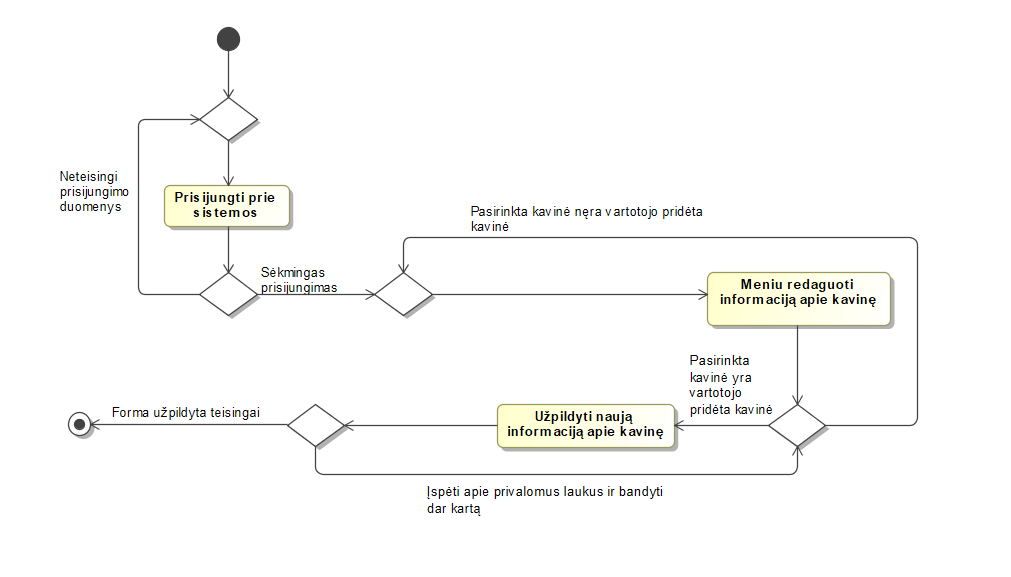
\includegraphics[width=\textwidth,height=\textheight,keepaspectratio]{img/editcafe} 
    \caption{Informacijos apie kavinę redagavimo veiklos diagrama}
    \label{img:editcafe}
\end{figure}
% Vietoj x įrašyt real sk.
x pav.   diagramoje nagrinėjami procesai, vykstantys vartotojui norint pakeist arba atnaujint informaciją apie kavinę. Norint redaguot kavinės informaciją, vartotojui būtina prisijungti prie sistemos. Vartotojas atidaro visų kavinių sąrašą ir pasirinkus savo kavinė ir paspaudus mygtuką "Show info" jis gauna informacija apie jo kavinę bei apačioje formą, kuria teisingai užpildžius ir paspaudus mygtuką "Change" galima atnaujint/pakeist egzistuojančią informaciją apie kavinę.

\section{Medžiagos darbo tema dėstymo skyriai}
Medžiagos darbo tema dėstymo skyriuose pateikiamos nagrinėjamos temos detalės:
pradinė medžiaga, jos analizės ir apdorojimo metodai, sprendimų įgyvendinimas,
gautų rezultatų apibendrinimas. Šios dalies turinys labai priklauso nuo darbo
temos. Skyriai gali turėti poskyrius ir smulkesnes sudėtines dalis, kaip
punktus ir papunkčius.

Medžiaga turi būti dėstoma aiškiai, pateikiant argumentus. Tekstas dėstomas
trečiuoju asmeniu, t.y. rašoma ne „aš manau“, bet „autorius mano“, „autoriaus
nuomone“. Reikėtų vengti informacijos nesuteikiančių frazių, pvz., „...kaip jau
buvo minėta...“, „...kaip visiems žinoma...“ ir pan., vengti grožinės literatūros
ar publicistinio stiliaus, gausių metaforų ar panašių meninės išraiškos
priemonių.

\subsection{Poskyris}
Citavimo pavyzdžiai: cituojamas vienas šaltinis \cite{PvzStraipsnLt}; cituojami
keli šaltiniai \cite{PvzStraipsnEn, PvzKonfLt, PvzKonfEn, PvzKnygLt, PvzKnygEn,
PvzElPubLt, PvzElPubEn, PvzMagistrLt, PvzPhdEn}.

\begin{enumerate}
	\item Pirmas elementas
	\item Antras elementas
\end{enumerate}

Lorem ipsum dolor sit amet, consectetur adipiscing elit. Curabitur at mauris sit amet nisi vestibulum tincidunt non vel mi. Pellentesque lacinia, sapien id sollicitudin egestas, diam erat dapibus justo, a cursus arcu nunc feugiat sapien. Mauris elit lorem, egestas at nisl at, consequat tempus nisi. Aliquam congue consectetur lorem ut venenatis. Suspendisse scelerisque eros ac sapien pulvinar, id fermentum sem bibendum. Phasellus rhoncus nec tellus quis gravida. Fusce at nibh porta, sodales ipsum quis, facilisis velit. Phasellus semper laoreet magna, eget eleifend massa. Donec sollicitudin risus risus, sodales dignissim ex bibendum et. Aliquam neque lectus, posuere vitae suscipit et, hendrerit eu mauris. Integer cursus neque ex, sed molestie ex suscipit et. Phasellus eget quam id arcu tincidunt fringilla eget eu tortor. In hac habitasse platea dictumst.



\subsubsection{Skirsnis}
\subsubsubsection{Straipsnis}
\subsubsection{Skirsnis}
\section{Skyrius}
\subsection{Poskyris}
\subsection{Poskyris}

\sectionnonum{Rezultatai ir išvados}
Šiame laboratoriniame darbe pasitelkiant skirtingus sistemos pjūvius aprašyta kavinių rezervavimo sistemos architektūra. Loginis pjūvis leido išskirti pagrindines esybes bei ryšius tarpjų. Kūrimo pjūvyje atlikta sistemos dekompozicija pradedant nuo bendro komponento toliaujį detalizuojant. Užduočių pjūvyje išsiaiškinti pagrindiniai agentų tikslai naudojantis sistema.Fiziniame pjūvyje apibrėžtas sistemos išdėstymas tinkle.  Galiausiai procesų pjūvyje išskirtiprocesai, jų komunikacija. Šis skirtingų požiūrių rinkinys leido iš ankstoaptikti sistemoje galimas klaidas bei sukurti tinkamą sistemos architektūrą.

%% PAKEISTAS PAVADINIMAS Į 'Šaltiniai'
\printbibliography[heading=bibintoc, title=Šaltiniai]  % Šaltinių sąraše nurodoma panaudota
% literatūra, kitokie šaltiniai. Abėcėlės tvarka išdėstomi darbe panaudotų
% (cituotų, perfrazuotų ar bent paminėtų) mokslo leidinių, kitokių publikacijų
% bibliografiniai aprašai.  Šaltinių sąrašas spausdinamas iš naujo puslapio.
% Aprašai pateikiami netransliteruoti. Šaltinių sąraše negali būti tokių
% šaltinių, kurie nebuvo paminėti tekste.

% \sectionnonum{Sąvokų apibrėžimai}
\sectionnonum{Santrumpos}
Sąvokų apibrėžimai ir santrumpų sąrašas sudaromas tada, kai darbo tekste
vartojami specialūs paaiškinimo reikalaujantys terminai ir rečiau sutinkamos
santrumpos.

\appendix  % Priedai
% Prieduose gali būti pateikiama pagalbinė, ypač darbo autoriaus savarankiškai
% parengta, medžiaga. Savarankiški priedai gali būti pateikiami ir
% kompaktiniame diske. Priedai taip pat numeruojami ir vadinami. Darbo tekstas
% su priedais susiejamas nuorodomis.

\section{Neuroninio tinklo struktūra}
\begin{figure}[H]
    \centering
    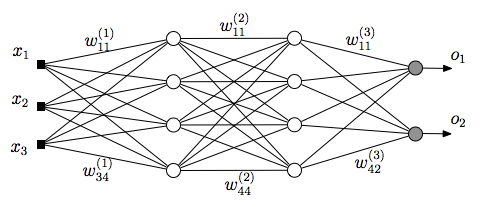
\includegraphics[scale=0.5]{img/MLP}
    \caption{Paveikslėlio pavyzdys}
    \label{img:mlp}
\end{figure}


\section{Eksperimentinio palyginimo rezultatai}
% tablesgenerator.com - converts calculators (e.g. excel) tables to LaTeX
\begin{table}[H]\footnotesize
  \centering
  \caption{Lentelės pavyzdys}
  {\begin{tabular}{|l|c|c|} \hline
    Algoritmas & $\bar{x}$ & $\sigma^{2}$ \\
    \hline
    Algoritmas A  & 1.6335    & 0.5584       \\
    Algoritmas B  & 1.7395    & 0.5647       \\
    \hline
  \end{tabular}}
  \label{tab:table example}
\end{table}

\end{document}
